\clearpage
\section{The figure for T3}

\subsection{The constraint nobody wrote down}

The obvious figure for a sensitivity analysis is a curve: the conclusion on one axis, the amount of
assumed knowledge withdrawn on the other, and a smooth frontier where the conclusion gives out. That
is the shape Rosenbaum's plots have, and it is the shape the paper's own figure rule went looking
for: a row whose interval stays flat for a while and then breaks.

That rule returned nothing. No query under the recovering set or under truthful knowledge has both
radii in the middle of the range on a network with real coefficients, and the rows that do have them
widen by a factor of twenty-seven to thirty-four before they break, so the plateau never happens.

The reason is in the data and it is the most important design fact here. The curve is not smooth.
It is a single step.

\begin{figure}[h]
\centering
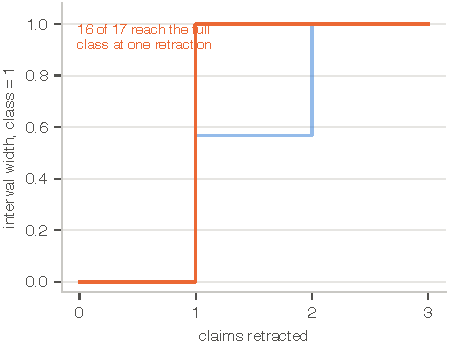
\includegraphics[width=.48\textwidth]{figs/f7_T3_steps.pdf}
\caption{Interval width against the number of claims retracted, one line per analysis, each
normalised to the width of the interval that uses no knowledge. Sixteen of the seventeen informative
analyses go from a point to the full class in one step. The exception is the textbook mediator,
which takes two.}
\end{figure}

Any figure that draws a frontier on this data is drawing something that is not there. The honest
encodings are the ones that treat the budget as what it is, a small integer, and put their effort
into showing what the step costs rather than pretending it is gradual.

\subsection{Five candidates}

\subsubsection*{F-A. The one-claim cliff}

Every analysis on one axis, each normalised so that the effect the analyst reported sits at one and
the null sits at zero. Three marks per row: the reported estimate, the interval after retracting one
claim, and the interval with no knowledge at all. The claim that does it is named in its own column.

\begin{figure}[h]
\centering
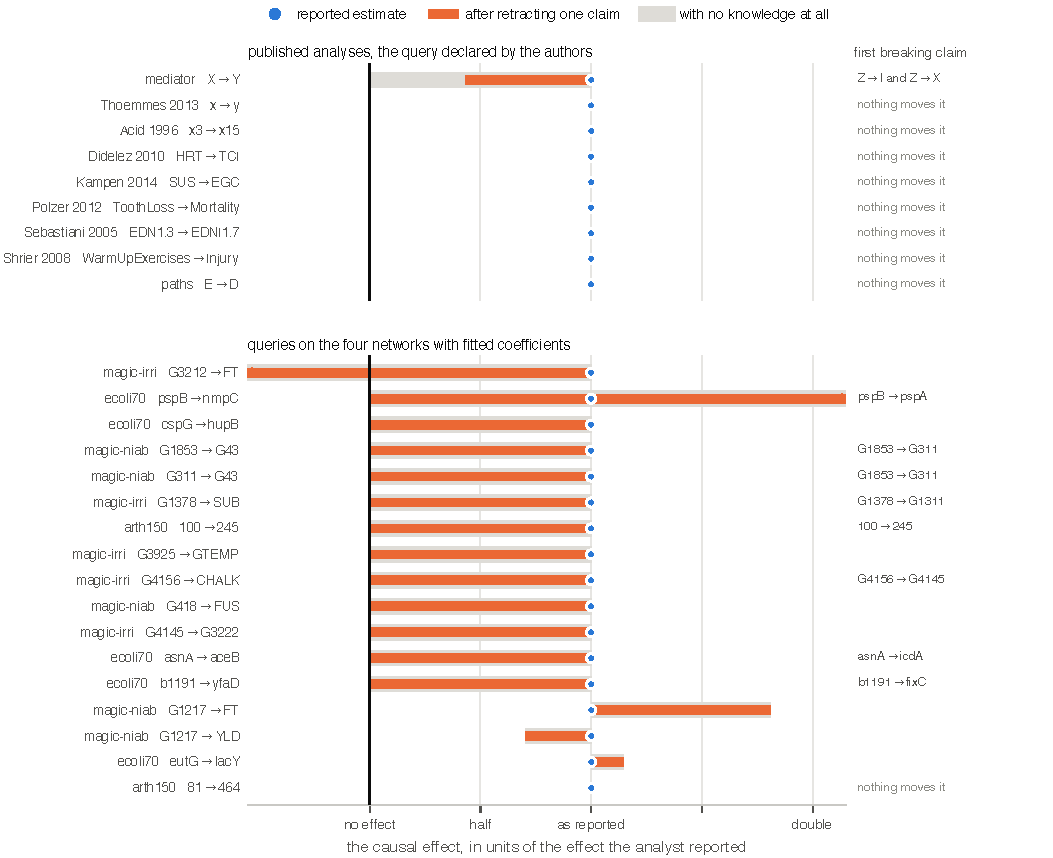
\includegraphics[width=\textwidth]{figs/f6_T3_dumbbell.pdf}
\caption{F-A, drawn from the twenty-six rows of T3. Normalising by the reported effect puts every
analysis on one scale and makes the pattern arithmetic rather than rhetorical: below the rule, one
retraction opens the interval from a point at the reported effect to everything between that and
zero. Where only the orange bar is visible, the grey one is underneath it, which is the finding.}
\end{figure}

What it shows: the reported effect and no effect become indistinguishable after one revision, on
every query drawn from the sampled frame, and on none of the queries the source papers declared.
Both halves are load-bearing and they sit in one picture.

What it costs: it needs a normalisation, and a reader has to accept that dividing by the reported
effect is fair. Two rows run off the axis and carry an arrow.

\subsubsection*{F-B. The step law}

The figure above, in the section on the constraint. Width against budget, one line per analysis.

What it shows: that the quantity is a step and not a frontier, which is the honest correction to
what a reader expects.

What it costs: sixteen of the lines are the same line. It is one fact, and a sentence carries it as
well as a panel does.

\subsubsection*{F-C. The state strip}

One row per analysis, one cell per budget, coloured by whether the interval at that budget still
determines the sign of the effect. No normalisation and no continuous axis, so nothing is implied
about magnitude.

\begin{figure}[h]
\centering
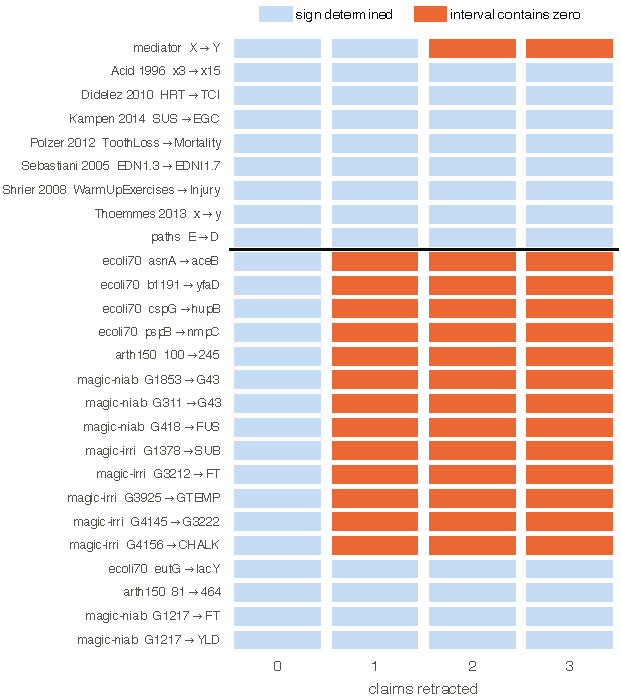
\includegraphics[width=.42\textwidth]{figs/f8_T3_strip.pdf}
\caption{F-C. The state of each conclusion at each budget, read from the stored null radius rather
than recomputed. Above the rule, the analyses whose queries the source papers declared.}
\end{figure}

What it shows: the discreteness, honestly, and the contrast between the declared queries and the
sampled ones at a glance.

What it costs: it drops the magnitude entirely. A reader learns that the conclusion goes and not
that it goes all the way to zero, which is the part that should alarm them.

\subsubsection*{F-D. The paradigm card}

One analysis, three lanes: what the analyst reports, what they would report having withdrawn one
named claim, and what they would report having asserted nothing.

\begin{figure}[h]
\centering
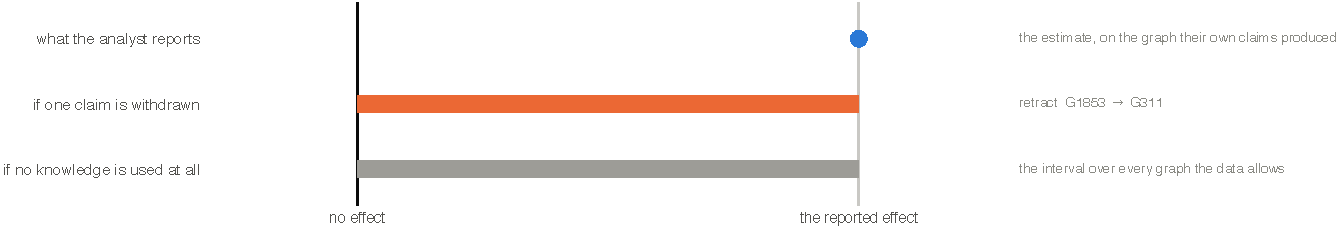
\includegraphics[width=\textwidth]{figs/f9_T3_card.pdf}
\caption{F-D. A single query on a network with fitted coefficients. The second lane and the third
are the same interval, which is what it means for the conclusion to rest on one claim.}
\end{figure}

What it shows: the object, the quantity and the sentence a practitioner would say, in one picture
that needs no axis labels to be understood.

What it costs: it is one row of a twenty-six-row table, so on its own it is an illustration. A
reviewer asks immediately whether it was chosen.

\subsubsection*{F-E. The cliff with its population}

F-A, with the distribution of the radius over every query in the corpus beside it, so that the named
analyses can be located in the population they were drawn from.

\begin{figure}[h]
\centering
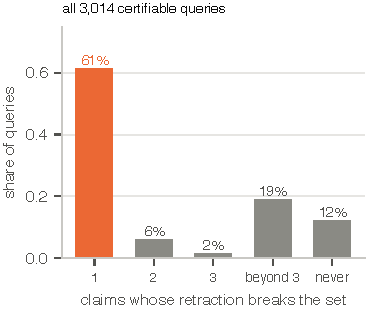
\includegraphics[width=.40\textwidth]{figs/f10_T3_population.pdf}
\caption{The right-hand panel of F-E: the breakdown radius over all 3{,}014 certifiable queries,
eleven knowledge conditions, 27 networks. The last two bars are queries whose set survives every
retraction the search reached, and queries no retraction can break at all. On 61\,\% of them the
committed set rests on a single claim.}
\end{figure}

What it shows: where the twenty-six named analyses sit in the population they were drawn from. They
are a selection, and the next section measures which of their columns that selection moved and which
it left alone.

What it costs: two populations in one float, which has to be said in the caption and read carefully.

\subsection{The recommendation}

\begin{verdict}
\textbf{Draw F-A, and put the population panel of F-E beside it.} Use F-D as the page-one teaser,
with a different query from the one F-A leads with, so the two do not restate each other. Keep F-B
as a sentence in the results and F-C in the appendix.
\end{verdict}

The argument for F-A over the others is that it is the only candidate that carries all three things
a reader needs at once. It shows the quantity, because the bar is the interval at one retraction.
It shows the consequence in the units the analyst reports in, because the axis is their own effect.
And it shows the comparison, because the grey bar behind is what they would have had with no
knowledge at all, and on sixteen rows of seventeen it is hidden underneath the orange one.

That last point is worth stating as the caption's one sentence, because it is the finding that the
table makes and the curve figure cannot: \emph{on these analyses, retracting a single claim returns
the analyst to the interval they would have had if they had asserted nothing}.

\subsection{Can this be the paper's main contribution}

It can be the main \emph{figure}. Two cautions before it becomes the main \emph{claim}.

The first is selection, and the next section measures it. The rows in the lower panel were chosen by
a rule that puts queries with a finite null radius first, so the null radius column of T3 is not
representative: 76\,\% of the printed rows against 43\,\% of the eligible ones. The width claim the
figure is built on is untouched by that rule, holding on 26 of 26 eligible queries and on 211 of 226
across the corpus. So the figure is safe and the caption must still say how the rows were drawn.

The second is that the figure is read as showing the null radius while the paper's headline quantity
is the breakdown radius. They coincide on most of these rows and they are different objects, and the one
analysis where they differ is the textbook one. A figure built on the interval reaching zero is
making a claim about conclusions; a figure built on the set ceasing to be valid is making a claim
about validity. Choose which, and say so in the axis label rather than in the text.

With both of those handled, the figure carries the paper. A reviewer who has read only the abstract
can look at it and see what the method measures, what it costs, and why the answer is uncomfortable.
